\documentclass[12pt,preprint,pdftex]{aastex}
\newcounter{address}
\newcommand{\project}[1]{\textsl{#1}}
\newcommand{\units}[1]{\mathrm{#1}}
\renewcommand{\mag}{\units{mag}}
\renewcommand{\arcmin}{\units{arcmin}}
\renewcommand{\arcsec}{\units{arcsec}}
\newcommand{\documentname}{\textsl{Article}}
\newcommand{\sectionname}{Section}
\newcommand{\sectionnames}{\sectionname s}
\newcommand{\rfifty}{r_{50}}
\newcommand{\rninety}{r_{90}}
\newcommand{\conc}{C}
\newcommand{\foreign}[1]{\emph{#1}}
\newcommand{\etal}{\foreign{et\,al.}}
\begin{document}

\title{
       The SDSS Large Galaxy Atlas
      }
\author{
        Ekta Patel\altaffilmark{\ref{CCPP}},
        David Mykytyn\altaffilmark{\ref{CCPP}},
        David W. Hogg\altaffilmark{\ref{CCPP},\ref{MPIA},\ref{email}},
        Dustin Lang\altaffilmark{\ref{CMU}}
       }
\setcounter{address}{1}
\altaffiltext{\theaddress}{\stepcounter{address}\label{CCPP} Center
  for Cosmology and Particle Physics, Department of Physics, New York
  University, 4 Washington Place, New York, NY 10003}
\altaffiltext{\theaddress}{\stepcounter{address}\label{MPIA}
  Max-Planck-Institut f\"ur Astronomie, K\"onigstuhl 17, D-69117
  Heidelberg, Germany}
\altaffiltext{\theaddress}{\stepcounter{address}\label{email} To whom
  correspondence should be addressed: \texttt{david.hogg@nyu.edu}}
\altaffiltext{\theaddress}{\stepcounter{address}\label{CMU} Carnegie
  Mellon University}

\begin{abstract}
We present the \project{Sloan Digital Sky Survey Large Galaxy Atlas}, which contains
accurate positions and photometry for galaxies with half-light diameter
greater than $1~\arcmin$. Galaxies of this size have rarely been measured with great accuracy. We present a table of measurements for such galaxies including their positions, colors, magnitudes, sizes, concentrations, surface brightness and axis ratios. Our input data has been taken largely from SDSS as well as the Third Reference Catalog of Bright Galaxies(RC3), the Two Micron All Sky Survey Large Galaxy Atlas and the NASA-Sloan Atlas.The measurement of galaxies with large angular sizes is challenging,
and has rarely been done well in automated settings.  Issues include
that the galaxies overlap field boundaries, overlap foreground stars,
and show detailed and confusing internal structure at high
signal-to-noise.  We take a generative modeling or likelihood approach
to making measurements of the galaxies, using very simplified
few-parameter morphological models and with the likelihood modified
for robustness.  We show that we can get precise and reliable (though
possibly biased) measurements of colors and surface brightnesses for
very large galaxies ($>1~\arcmin$ in diameter) in the \project{Sloan
  Digital Sky Survey} imaging data. We specifically highlight those large galaxies which have not been found in RC3, but, have been included in the NASA-Sloan Atlas with $50\%$ light radii $> 30\,\arcsec$. Some examples of these include galaxies from the Messier catalog which have been measured as large as $\sim 260\,\arcsec$ while retaining accurate galactic properties. We have stopped at $\sim 260\,\arcsec$ for matters of necessity with regards to future projects.

\end{abstract}

\section{Introduction}

The \project{SDSS} never made good photometry for the brightest galaxies because it oversubtracts the sky for very large objects, but it did make beautiful images. The Nasa-Sloan Atlas(NSA) rephotometered all redshifts for galaxies within the SDSS Data Release 8. It takes the images from the \textit{ugriz} bands of SDSS and the NUV and FUV bands from \textit{GALEX}.\footnote{\url{www.nsatlas.org}} The methods used in the NSA is an improvement to those used by SDSS. It begins with and estimation of the sky from an processed SDSS image and creates masks for all bright sources in and around the image. A spline is fit to the unmasked data with constraints that make the process run even for images where heavy masking is needed \citep{blanton11}. 
% how does NSA improve the SDSS background? What is the SDSS method? How do we correct for sky using tractor?

The RC3 catalog, which contributes the most galaxies to our data set, gives methods of measurements in Volume I of the catalog. Positions for the galaxies contained in RC3 were measured using the SAO Star Catalog and the FK4 coordinate system, but are listed by the 2000.0 equinox positions. A large number of positions were also taken from the CGCG, UGC, and MCG catalogs. $D_{25}$ was measured at the 25.0 B-m/ss level in units of 0.1 arcminutes. The isophotal diameters are largely taken from three sources including derivations from de Vaucouleur's photoelectrically calibrated photographic and CCD photometry, interpolation of R.Buta's photoelectric growth curves, and from the photoelectric calibration of surface photometry by Lauberts and Valentijn from which the largest contributions are made to RC3's $D_{25}$ values. Galactic extinction was measured using the Burstein \& Heiles method, which involves a combination of local galacatic HI column densities and faint galaxy counts. Internal extinction is measured by \begin{equation} A_i= \alpha(T)log(R_{25}) \end{equation} where $\alpha(T)$ is a coefficient dependent on morphological type and $R_{25}$ is the axis ratio. Various magnitudes were measured and included in the RC3 catalog. The total photoelectric magnitudes, $B_T$, were found using two methods which are the extrapolation of photoelectric aperture photometry using standard curves and the extrapolation of the calibrated surface photometry. Two different surface brightnesses are included. One measures the mean effective surface brightness with the effective aperture, $A_e$. The other method measures the mean surface brightness within the $D_{25}$ ellipse, using the the axis ratio,$R_{25}$\citep{rc3}.

The 2MASS Large Galaxy Atlas(LGA) provides near-infrared photometry for large galaxies to connect the gap between optical wavelengths and longer wavelengths. We have checked for galaxies in the LGA that were not included in RC3 down to a radius of $1\arcmin$, which was the lower size limit for galaxies included in this catalog. The radius measurement in 2MASS was based on the K-band isophotal properties \citep{jarrett03}.  

The \textit{GALEX} Ultraviolet Atlas of Nearby Galaxies provides photometry, surface brightness and color profiles for 1034 nearby galaxies with a diameter larger than $1~\arcmin$ and a surface brightness in the b-band, $u_B$=25 mag arcsec$^{-2}$ . The galaxies chosen for this data set come from the \textit{GALEX} Nearby Galaxies Survey and other equivalent\textit{GALEX} initiatives that viewed the same fields of the sky in the far-ultra violet(FUV) and near-ultra violet(NUV) bands. All galaxies with a diameter larger than $1~\arcmin$ from RC3 were also added to the sample. A total of 81 out of 1136 galaxies were not included in the Atlas because they were in regions of very high background, high Galactic extinction, extremely low UV surface brightness, or simply had images that were not of sufficient quality for analysis. The surface brightness was measured using the central position, ellipticity, and position angle of the D25 ellipse. It is computed to within the annuli of ellipse's central angle increasing out by $6~\arcsec$ from the major-axis until it reaches at least 1.5 times D25. Point sources in the images with colors redder than FUV-NUV=1 were automatically masked and visually checked. After the SExtractor-detected sources were masked within a 5x5 pixel range of each source, the mean of the sky was used as the estimate of the background due to low background in FUV. Galactic color excess is taken from \cite{schlegel98} and used with the extinction law from \cite{cardelli}. The surface brightness profiles were then used to compute asymptotic magnitudes, colors, luminosities and concentrations. Magnitudes, effective radii, and colors were found by extrapolating growth curves to infinity and performing error-weighted linear fits. The morphology of the UV surface brightness profiles were determined visually using a two-letter naming scheme, the first describing the outer profile and the second describing the inner profile \citep{gdp06}.

%HOGG: discuss general issue that our photometry is being done the way it is to meet particular goals

\subsection{Methods Intro}
The \project{Sloan Digital Sky Survey} (\project{SDSS}) and its
successor projects \project{SDSS-II} and \project{SDSS-III} have had
enormous impact, forming the observational basis for literally
\emph{thousands} of refereed papers.  The success of these surveys can
be attributed to multiple factors, not least the unaccountable
diversity of phenomenology presented to us by our fecund Universe.
One significant factor has been the fact that these surveys have
endeavored to produce and distribute (to the public) reliable,
calibrated, easy-to-use photometric and spectroscopic data.

All that said, the goals of the \project{SDSS} were heavily weighted
towards galaxies and stars with visible brightnesses around 18~mag.
The camera, observing strategy, and data-reduction pipelines were all
optimized for performance at 15 to 22~mag.  Importantly---and to the
chagrin of some investigators (CITE SOMETHING)---the \project{SDSS}
photometry of very bright, nearby galaxies has been substantially
biased.  The dominant reason for this is that the \project{SDSS-I}
photometric pipelines employed an ``aggressive'' sky estimation
algorithm that removed much of the light from sources with large
angular footprints.  A secondary reason is that the ``deblending''
heuristics for disentangling the light in overlapping galaxies don't
deal well with sources that are hundreds or thousands of times the
solid angle of the core of the point-spread function.

The nearby galaxies are interesting and important!  Because the
\project{SDSS} is supremely well calibrated photometrically, and
because it is a drift-scanning survey, it is particularly well suited
to measuring these objects with large angular extents.  In this
\documentname, we make an attempt to photometer some nearby galaxies
in the \project{SDSS} imaging data and test the precision of those
measurements.

This project has been made possible by two developments.  The first is
that for \project{SDSS-III}, a new global, continuous sky function was
fit to the imaging data, fit to the ``blank'' pixels (CITE BLANTON).  This sky
function does not remove light from large galaxies, or not nearly as
much as previous generations of sky algorithms.  The second is that we
have developed a package \project{The Tractor} (HOGG CITE) for fitting
probabilistic models to astronomical imaging data and the
\project{SDSS} imaging in particular.

In what follows, we fit \project{SDSS} imaging
data on and near large angular-size galaxies using simple (inflexible)
models---mixtures of exponential and de~Vaucouleurs models.  For each
galaxy, we use \project{The Tractor} to
optimize a justifiable scalar objective function that is an
approximation to a likelihood, with modifications to make the fitting
less sensitive (than traditionally) to outliers and morphological
oddities in the galaxies.  The galaxies are typically as large as or
larger than an individual \project{SDSS} frame, but \project{The
  Tractor} doesn't need a co-add or mosaic of the data; it fits all
the individual disjoint science exposures simultaneously.  For most
galaxies we look at, the simple models we are using are \emph{not}
good fits: They can't be, because they don't capture spiral arms, HII
regions, dust lanes, or other morphological non-trivialities.
However, as we will show, they produce precise, robust photometry that
appears to be invariant with galaxy angular size or distance.

Readers who don't want to read the long philosophical position
outlined in \sectionname~\ref{sec:philosophy} can skip either to the
data and method descriptions in \sectionnames~\ref{sec:data} and
\ref{sec:method} or else straight to the results in
\sectionname~\ref{sec:results}.  There is a short final discussion in
\sectionname~\ref{sec:discussion}.

\section{Data and input catalogs}

%Hogg: Stuff about the \project{SDSS} imaging ...

The initial input catalog was formed out of the union of the Third Reference Catalog of Bright Galaxies (RC3), the NASA-Sloan Atlas (NSA), and the 2MASS Large Galaxy Atlas (LGA). Objects were searched for in those catalogs with an angular diameter greater than or equal to two arcminutes. For the Third Reference Catalog the cut made was based on the measured apparent major isophotal diameter of the surface brightness $\mu_{B}$ greater than 1 arcminute. For the NASA-Sloan Atlas, we checked for any objects of significant size that were
also not in RC3. The cut was for objects with a 50\% light radius of
the SERSIC fit greater than 30 arcseconds. The objects were then
examined by eye to determine which ones were actual large galaxies,
and which were errors in the NSA. Example errors included stars
causing saturation, interstellar medium, and nebulae. Some interesting galaxies that were not contained in RC3 were found and measured and have been included in the Atlas. Some of these images contained two galaxies, which we fit individually. We also checked
the 2MASS Large Galaxy Atlas but no galaxies of the correct size not
already in RC3 were found. The only objects found were either not in
the Sloan Survey, or were globular clusters. The cut for 2MASS was
based on the isophotal fiduciary radius in the K-band, which was
checked to a radius of 1 arcminute.

\subsection{Method Data and Input}\label{sec:data}
The imaging data for this project come from the \project{Sloan Digital
  Sky Survey} fully public \project{Data Release 8} \citep{dr8}, which is
the first data release of the \project{SDSS-III} project \citep{sdssiii}.  It
includes fully recalibrated imaging \citep{padmanabhan} from the
combined imaging projects of \project{SDSS} \citep{york}  and
\project{SDSS-II} \citep{sdssii}.

...key point is the new sky...

The fitting code (\project{The Tractor}, described briefly below, and
more completely in Lang \etal, forthcoming) locates \project{SDSS}
imaging fields that overlap a large circular footprint centered on the
pre-fitting (input) galaxy center.  It downloads (on the fly)
\project{DR8} imaging data files corresponding to those fields from
the \project{SDSS-III} \project{Data Archive Server} (CITE?).  The
downloaded data files are the photometrically calibrated,
background-subtracted ``frames'' files.

For every pixel of the imaging, we construct an approximate ``inverse
variance'' value, which is the reciprocal of the variance expected
given the Poisson photon, Poisson dark-current, and Gaussian
read-noise error models.  In detail, we use the equations recommended
by the \project{SDSS-III}
Collaboration.\footnote{\url{http://data.sdss3.org/datamodel/files/BOSS\_PHOTOOBJ/frames/RERUN/RUN/CAMCOL/frame.html}}
We set the inverse variance to zero for any pixels that lie in regions
that were interpolated, saturated, or affected by cosmic rays or ghost
images.

For the PSF model, we use the SDSS double-Gaussian model stored in the
``psField'' file.  DSTN: What do we get as parameters for that
double-Gaussian model?  I think it is less than 1 + 4 + 6 parameters
that a K=2 D=2 MoG would have, right?

Galactic extinction $E(B-V)$ values are taken at the galaxy center
positions from the standard maps (\citealt{schlegel98}).  The
reddening values are then multiplied by the appropriate coefficients
A(V)/E(B-V) per Sloan bandpass to obtain the total extinction to be
subtracted from the individual magnitudes of each bandpass. The
coefficiens are the following: u-5.155,g-3.793, r-2.751, i-2.086,
z-1.479.

In this paper we use a sample of galaxies for testing which we do not
intend to be complete.  The source for this sample---which is only
really bringing initial (or first-guess) celestial positions---was the
Third Reference Catalog of Bright Galaxies \citep{rc3}.  From this
catalog we used only objects with angular diameter measured in the
apparent major isophotal diameter at the surface brightness level
$\mu_B = 25.0$~mag in 1~arcsec$^2$ arcsecond of [DM WHAT SYMBOL?]
$>1$~arcmin.

\section{Method}
\subsection{Galaxy photometry is impossible}\label{sec:philosophy}

There is a deep sense in which obtaining precise and accurate galaxy
photometry is fundamentally impossible.  The reasons are multiple, but
the dominant reasons are, first, that the angular outskirts of
galaxies can contain significant luminosity but at incredibly low
surface brightness and unknown morphology, and secondly, that the
imaging point-spread function (PSF) can also have large-angle
contributions that are unknown.  The latter problem affects stellar
photometry also, but so long as the PSF is constant, precise and
accurate stellar photometry \emph{is} possible.  The difference
between galaxies and stars is that all point-like stars will
illuminate the PSF (correlate with it) identically.  Stellar
photometry does not rely on getting all this right so long as it deals
with it \emph{consistently} across stars.  Not so for galaxies, each
of which might have very different correlations with the PSF at large
angles.  There is no way to produce consistent photometry without
knowing things about every galaxy and every PSF that are---almost in
principle---unknowable.

These fundamental issues and also many pragmatic issues of noisy,
badly calibrated, and crowded imaging have forced astronomers to
consider many different methods for measuring galaxy fluxes.  Each has
flaws.  Here we give a highly biased and very brief review.
\begin{itemize}
\item Given digital imaging of a patch of sky that includes a galaxy,
  the simplest way to measure the flux of that galaxy is
  \emph{aperture photometry}.  This is the measurement of the total
  light (the integral of the intensity, found by summing pixel values)
  in the image above the sky (foreground and background) intensity
  within a fixed circular angular aperture, centered on the galaxy.
  This kind of photometry obtains different fractions of the galaxy
  light in galaxies that have different proper sizes or which lie at
  different radial (angular-diameter) distances; in this sense it
  doesn't produce photometry that is distance-independent.  It has
  many other problems as well, some of which will come up later in
  this list.
\item Aperture photometry can in principle be improved by scaling the
  radius of the aperture with the inverse radial (angular-diameter)
  distance to the galaxy.  This helps in making the photometry
  distance-independent, but it requires prior knowledge of the galaxy
  distances.  It also doesn't perfectly compensate for distance
  because galaxies at different distances but subject to the same (in
  angular size) PSF illuminate even the properly scaled apertures
  differently.  This change also doesn't account for galaxies with
  different proper sizes.
\item Aperture photometry can be made adaptive, adapting the aperture
  to the observed angular size of each galaxy.  This requires image
  analysis---galaxy size measurement---prior to the photometry.  In
  one extreme version, \emph{Isophotal photometry}, the photometric
  aperture is made the (usually very non-trivial) precise \emph{shape}
  of a particular intensity contour in the galaxy image.  Isophotal
  photometry is close to distance-independent for low-redshift
  galaxies; at high redshift relativistic intensity dimming
  ($[1+z]^{-4}$) breaks that symmetry.  Also, isophotal photometry
  will in general get very different fractions of the galaxy light
  from high and low surface-brightness galaxies.  It also remains at
  least slightly dependent on the PSF for the same reasons as the
  previous methods.
\item \emph{Petrosian photometry} \citep{petrosian} adapts the angular radius of
  the photometry aperture using a statistic of the galaxy profile that
  is insensitive to total surface brightness.  It works by identifying
  a radius at which the (azimuthally averaged) intensity is a fixed
  fraction of the mean within that radius.  Again, this method is at
  least slightly dependent on distance, again because of the PSF.
\item The most adaptive methods in common use---not the most adaptive
  \emph{possible}---involve measuring the galaxy's \emph{radial
    profile} by averaging the intensity above the sky intensity in
  narrow circular (or sometimes elliptical) annuli centered on the
  galaxy, and then summing the annular contributions to the flux, and
  maybe also extrapolating at large radius.  These methods are usually
  designed to attempt to get ``all the light''.  They do not overcome
  the fundamental problem of large-radius galaxy and PSF morphology.
\item One problem in common to all the above approaches is that they
  involve ``adding up'' the flux in pixels.  This arithmetic operation
  creates what is classically called a ``statistic'' of the data; it
  will not be the minimum-variance estimator of anything.  That is, if
  information preservation or precision is of high value, none of the
  above methods are palatable.  Information-preserving inference
  requires fitting probabilistic models, with a likelihood funtion at
  least and maybe also informative priors.  In the enormous
  \project{Sloan Digital Sky Survey}, despite the fact that aperture
  and Petrosian magnitudes were measured and published, it was the
  magnitudes based on \emph{model fitting} that got the most use: They
  produced more precise colors.  It is also the case that model
  fitting is the first method in this list that has a shot at
  producing truly distance-independent measurements, because a
  component of the model fit is the PSF.  Inasmuch as the galaxy and
  PSF models are appropriate and correct, model fitting is in some
  sense provably the best way to measure galaxy photometry.  Of course
  it doesn't overcome the fundamental problems of galaxy photometry
  with which this \documentname\ opens: We don't understand galaxy
  profiles or the PSF at large angular radii, and though there can be
  significant light out there, it is hard to find in the data.
  Furthermore, in the standard methodologies of model fitting,
  extremely simple galaxy models are used, such as elliptical
  exponentials and de~Vaucouleurs profiles \citep{dev}.  These smooth
  models are not at all a good description of two-dimensional images
  of most real galaxies at \emph{any} angular radius (think: spiral
  arms, bars, rings, HII regions, dust lanes, and so on).
\item An almost unexplored territory for galaxy photometry is to
  consider extremely flexible galaxy models, models so flexible that
  they can capture all of the details.  This would require a
  significant technical investment and a lot of computer time, but it
  might pay off.  It ought to give the best measurements in the end;
  it is the ultimate in ``letting the data decide''.  However, even
  this flexible approach won't overcome the fundamental problems; in
  some sense the true, total photometry of a galaxy is \emph{not an
    observable}.
\end{itemize}
All the problems with these different photometric measurement
techniques flow into the subsequent or simultaneous measurements made
of other quantities of interest, like sizes, concentrations, surface
brightnesses, and so-on, because these measurements are (or involve)
transformations of photometric measurements.  The best choice among
techniques will depend on the uses to which the measurements are going
to be put; in some cases precision is paramount, in others consistency
across distance, in others robustness to varying PSF, in others
consistency across morphological types.

In this project, our goal is to obtain consistent multi-band
photometry for a large set of galaxies at a wide range of distances,
with a large range of morphologies, surface-brightnesses, and angular
sizes relative to the PSF.  Importantly, we want to do the very
(angularly) large galaxies in the same way as we do the (angularly)
compact.  Consistency is more important than accuracy, in the sense
that we would like to get numbers that---if they must be wrong---are
wrong \emph{in the same way} for the \emph{same galaxy} observed at
different distances or through different atmospheric PSFs.  We also
want precision---we want to avoid introducing unnecessary scatter or
noise by our choice of procedure.

These considerations argue \emph{for} probabilistic modeling and
\emph{against} using very flexible models.  We are making a catalog of
photometry, not delivering posterior PDFs; our photometry will
therefore contain \emph{estimators} for flux, color, size, and so-on.
Minimum variance estimators are maximum-likelihood estimators, so we
will only consider approaches in which we (under assumptions)
construct an approximate likelihood function and optimize it.  As we
note above, the requirement that our photometry be distance and
PSF-independent also argues for modeling approaches.  The reason we
prefer inflexible models to flexible models is that at the optimum in
the likelihood, a large angular-size galaxy will exercise much more
model freedom than a small angular-size galaxy: In the large galaxy,
many more features and details are visible under finite PSF.  Again,
distance and PSF consistency requires that we restrict model freedom
identically or as identically as possible for all galaxies we measure.
This argues for overly simplistic models; the models we will use below
do \emph{not} capture the full two-dimensional structure of the
galaxies being measured, but (as we will show), they do provide
robust, high signal-to-noise, consistent measurements.

In addition to the photometric issues discussed above, there are a
large number of separate pragmatic issues when we consider the problem
of performing galaxy photometry automatically and consistently in a
large and heterogeneous data set.  When galaxies are angularly large,
as they will be here, they often overlap stars.  Bright stars make it
hard to precisely measure the fainter galaxy.  Faint stars are
challenging to deblend from the galaxy reliably.

In addition to overlapping stars, galaxies frequently overlap other
galaxies, both because galaxies are spatially clustered and because
some ``galaxies'' are really pairs of galaxies merging.  Overlapping
galaxies must be ``deblended'', which is a source of consternation in
many imaging surveys.  The consternaton arises both because proper
deblending is an ill-posed problem and because it is very
distance-dependent.  The problem is ill-posed because there is no
definition of the boundary between two galaxies and one; even if there
were, we wouldn't know how to separate the observed intensity into the
two components.  Clever data-driven heuristic proposals and methods
exist (cite Lupton and SExtractor) but nothing is reliable for
angularly large galaxies, where enormous non-smooth detail is visible
for a large range of Hubble types.  Deblending is distance-dependent,
because a galaxy observed nearby is much larger than the PSF; all of
the spiral structure and HII regions are well resolved.  A distant
galaxy is a smooth blob under the PSF.  The deblending simply can't be
the same if it is based on flexible heuristics.  This is another place
where fitting inflexible models will help us: Although the inflexible
models are never good fits, they provide objective methods for
simultaneously measuring two overlapping galaxies.

\subsection{Measuring Galaxies}

...first a few words about \project{The Tractor}

Models: Write about the types of models used?? Different galaxies types etc?
The Tractor functions first by building a model, using initial parameter data that is supplied. Next, it takes the derivative of each parameter and performs a weighted least-squares fit to find a parameter update that will minimize $\chi^2$.  Since this is a linearization of a non-linear problem, we perform a line search along the update direction, taking steps of increasing size starting from $1/1024$ and increasing by factors of $2$ up to a factor of $2$ of the linear direction; we halt the line-search when the $\chi^2$ stops decreasing.  Finally the parameters are updated in that direction. The tractor is capable of freezing certain parameters, so that they are excluded from the optimization. 
The iteratively-reweighted least squares process is used to update the
inverse variances after each iteration of optimization. The math is:
\begin{eqnarray}
\chi^2 &\equiv& \sum_n \chi_n^2
\\
\chi_n^2 &\equiv& \frac{[d_n - m_n]^2}{\sigma_n^2}
\\
\frac{1}{\sigma_n^2} &\leftarrow& \frac{1}{\sigma_n^2}\,\frac{Q^2}{Q^2+\chi_n^2}
\quad ,
\end{eqnarray}
where $Q$ is the number of ``sigma'' at which the residual saturates. $Q$ for these fittings was chosen to be 5. (Find out why)

In order to deal with the problems of stars that overlap with the
galaxy which we are interested in, we decided to mask them out. The
stars were found using the data in the Tycho-2 star catalog \citep{tycho2}.
The stars were masked out to a
radius of
\begin{equation}
\theta_{\mathrm{exclude}} = \max(25, 25\,2^{[11\,\mag-V]})
\end{equation}
where $V$ is the visual magnitude given by Tycho-2.
(I'm not sure why these values, I got them from Dustin) The mask was applied by setting the chi values of the masked out pixels to zero.



...now the specifics of what we actually do

When given an RA and a Dec and a radius, the program searches the SDSS data for fields which overlap anywhere in that space. It downloads all those fields, in all bands, as fits files, and then imports them into the program as arrays. The initial inverse variances are also downloaded from Sloan.
Saturated pixels from the SDSS images were masked and then a binary dilation with three iterations was applied. (more details needed here?)

For the purpose of measuring and optimizing on a single galaxy at a
time, all other objects were removed from within a circle centered on
the galaxy center and radius, both given by the RC3 catalog (using the major isophotal diameter)
 for that particular catalog. This was done rather than
working within the SDSS catalog because SDSS frequently splits up large
galaxies into numerous small ones and so it was much easier to simply
start over with a single galaxy. As initialization, that galaxy was
given magnitudes of 15 in every band and a radius given by the RC3
catalog.


We start the fitting with an exponential galaxy and then optimize
simply that galaxy six times. Following that, we switch to a composite
galaxy, with both exponential and deVaucouleur components. These
components are free to vary separately in order to best fit the
data. This new composite galaxy is also optimized six times by itself.

In order to measure the half-light radius $\rfifty$, the 90 percent
radius $\rninety$ and the concentration parameter $\conc\equiv
\rninety/\rfifty$, we took the model of the galaxy that had been
optimized and places it in an empty frame within the tractor. Next,
over a series of increasing intervals of radii we summed up the total
flux within the circles and then interpolated to find $\rfifty$ and $\rninety$.
 We used sixty-four radii equally spaced in pixel logarithms from zero
 to half the height of the image. Exceptional cases were flagged for later
 review if $\rfifty$ was not between the deVaucouleur and exponential radii
 for that galaxy, and concentration was flagged as incorrect if $\frac{1}{\conc}$
 was not between .29 and .46. (We are not getting these numbers, mention in
 discussion?) TODO: Add citation to paper for these numbers.

An example of the finished result is given for NGC 4605, which had 6 fields that combined to make our image. These six are shown separately here. In fig \ref{fig:4605data} the data from these fields are shown in the i-band. Fig \ref{fig:4605model} shows our completed model for this galaxy. Fig \ref{fig:4605diff} is the difference between the data and the model. Finally \ref{fig:4605chi} shows our chi values for the galaxy. Fig \ref{fig:colorsdata} shows the different data for each band, and figs \ref{fig:colorsmodel}, \ref{fig:colorsdiff}, \ref{fig:colorschi} shows the results for the model, the difference between the model and the data, and the chi values.


\subsection{Creating the Catalog}

For the largest of galaxies, SDSS provided many fields where each field contained images in each of the \textit{ugriz}. Examples of these include the Messier galaxies. For those galaxies which had between 10 and 20 images, the pixels in the images were scaled down by a factor of 2. Galaxies with 20 to 40 images each were scaled down by a factor of 4. Galaxies with 40 to 80 images were scaled down by a factor of 8 and those with more than 80 images could not be run through the \textit{Tractor} successfully. The binning of the pixels in these images did, however, provide sufficient accuracy to within a few percent for the colors in comparison to colors resulting from no binning. Other cases of galaxies that had to be treated specially include those in which there was a pair of galaxies in one image. These scenarios were manually measured as two individual galaxies. Some examples include M51 and the Mice Galaxies in which cases the secondary measurements seemed to be within a few percent error of the dense region in the color-color plot in Figure 2(are we plotting these on the color-color to show it?). Another special case is that of a bright star whose masking caused a part or whole of the galaxy to be masked with it. In some cases, these were re-run manually, while those in which the whole galaxy was masked were discarded.  Additionally, we observed those cases in which galaxies were off-center in the images and re-ran those manually with an initialization beginning at the center of the galaxy rather than the center of the image. 

With the raw results from the $Tractor$, we first applied extinction corrections as given by Schlegel et al. 1998 using the \textbf{astropysics} package.\footnote{\url{packages.python.org/Astropysics}} The get\_sfd\_dust function in the obstools module of the {\bf astropysics} package allows us to retrieve the reddening value E(B-V) from the dust maps by converting the RA and Dec that we measure to galactic coordinates. The reddening values are then multiplied by the appropriate coefficients A(V)/E(B-V) per Sloan bandpass to obtain the total extinction to be subtracted from the individual magnitudes of each bandpass. The coefficients are the following: $u=5.155,\;g=3.793,\; r=2.751,\; i=2.086,\; z=1.479$. With the corrected magnitudes, we were then able to compute surface brightness with \begin{equation} \mu_{50,i}=m_i+2.5log(\pi{r_{50}}^2) \end{equation} where $m_i$ is the corrected magnitude in the i-band and $r_{50,i}$ is the half-light radius in the i-band. For a description of how the radii, concentrations, magnitudes, and axis ratios were computed see the methodology in Mykytyn et al. 2013. 


%A few examples showing what works and what doesn't ...

\section{Catalog}
The table of data contains the RA, Dec, and name given by each galaxy's source catalog(RC3 or Nasa-Sloan Atlas).For the measured positions of all galaxies included in the Atlas, see Figure 1. The data from the composite galaxies includes the RA, Dec, magnitudes, half-light radii, colors, etc. See Table 1. Those galaxies which wehave denoted with flags can be found in the exceptions table. See Table 2. 

%insert exceptions table and snippet of our final atlas

\subsection{Hand-Vetting}
We have made various visual checks on our galaxies, which have led to a number of manual reruns for improved measurements. In some cases, the second result provided more valuable measurements, while in others, the rerun did not seem to improve the original measurements. For a full list of our comments from visual inspections, see Table 2. One of the first interesting selections that we chose to inspect was a set of all objects that came from the NASA-Sloan Atlas and contained a radius larger than 30 \arcsec. We chose to observe these objects because we only chose objects from NASA-Sloan that did not already belong to RC3. In many cases, the galaxies were being obstructed by large stars in the same field as the galaxy, causing saturation of the image and imporper measurement of the galaxy overall. Other galaxies, however, such as NSA ID 148151 have proven to results in a good fit. Others were simply groups of galaxies, each too small individually to fulfill the size criteria for our catalog. Lastly, there were some irregular galaxies with very low surface brightnesses.

%Optical images were created for the preliminary atlas objects using the g,r,and i band photometry. These were sorted by increasing half-light i-band radius. At this stage, the images and the consequent flipbooks of measurements were observed for galaxies which seemes to be flaw in one of the following ways: groups or pairs of galaxies that should be individually run, galaxies that were off center, fields of the sky that appeared to contain no galaxy, or galaxies with bright stars nearby or overlapping with the image of a galaxy. Notes from this visualization were compiled and combined with those of objects with infinite i-band flux. 

Another set of galaxies that was observed individually by eye were those which had an infinite i-band flux. Many of these images had bad sky levels in the i-band as well due to groups of galaxies or stars in the vicinity. Other fits were not initializing in the correct place for galaxies that were not in the center of their fields. For those, we reran our fits giving an intial position for the fit to measure from, which in most cases improved the measurement enough to discard the original fit. This set of galaxies also contained candidates that simply did not produce good fits because of a large bright star in the background or foreground of the galaxy.
%Hogg:Do we want to give examples of both a bad one and one that was able to improve through manual tweaking or should we direct them to the method paper?

Galaxies that were outliers on a plot of half-light i-band surface brightness and g-i color were investigated as well. In the case where two galaxies were in the same field, we measured each galaxy individually. For merging galaxies, most pairs led to good fits for each galaxy individually despite the lack of explicit boundaries between the merging galaxies. NGC 3395 and NGC 3396 are an example of a merging pair of galaxies that were measured well. Pairs of galaxies that are not merging, however, were not as succesful overall. For some pairs, the individual measurement of one galaxy overtook the fit of the second galaxy, causing innacurate measurements. An example of a bad fit of a pair of galaxies is NGC 4649 and NGC 4647. For pairs that did not run as two separate succesful galaxies, we only include the galaxy that has a better fit. The rest of the outliers in this investigation of our fits were galaxies whose measurements did not initialize at the location of the galaxy due to the galaxy being off-center in its field. For these galaxies, new position parameters were given using the NASA/IPAC Extragalactic Database. A majority of these galaxies showed significant improvements in their new measurements. In all cases where a galaxy was an outlier on the surface brightness versus g-i color plot, the new measurement was accepted as good and the original measurement discarded unless otherwise noted in Table 2.

Two pairs of galaxies that were rerun as two individual galaxies included companion galaxies that were not included in either NASA-Sloan or in RC3. The companions are NED 01, found next to NSA ID 86994 and PGC 1563523, which is found with NGC 52. The companions have not been included in our table. 

The last method used to do a visualization check on the galaxies was a sorting of the galaxies by g-i color into quartiles. A cut was made at the 50th percentile of the data and again at the 25th and 75th percentiles. Each of these quartiles were further split into four more quartiles each by half-light surface brightness in the i-band. We now have a data set that is divided into 16 subsets by color and surface brightness. They were labeled such that the bluest and highest surface brightness galaxies are flagged with a 0 and then reddest and lowest surface brightness galaxies are flagged with a 15. Again, images using the g,r, and i band photometry were created sseparetly for each of the 6 subsets of data, this time ordered by decreasing 90\% light radius. With these images, we made comments on galaxies that did not fit the size order criteria and observed the details of their measurements. In many cases for galaxies that appeared to be smaller than their measured radius, the fits were extending too far away from the center of the galaxy structure. In some other cases, nearby stars were being over-masked and consequently masking pieces of the galaxy in that field. 


%include a diagram here of the way we labeled 0-15? finish writing once we have decided what to do with them

%Hogg: Will we want to add those two companions in manually to the atlas even though they won't have 'source' information from NSA or RC3?

%Hogg: Are we including the plot of sb and color with our hand drawn line of it to show what we mean by outliers?

%Ekta: add process of splitting up quantiles and making comments on those galaxies
\subsection{Exceptions and issues}\label{sec:results}
For instance, the galaxy M81 had too large of a radius in RC3 in order to run properly so it was manually reduced so as to fit into the memory of the machine. The scaling factors used were if the number of fields were between ten and twenty, a factor of two scaling. Four was used for between twenty and forty, and eight was used for between forty and eighty. Above eighty, the galaxy was skipped. (Put into table?) Another example is M51a and M51b, which were simultaneously fit in order to ensure that the fit measured both galaxies simultaneously. 

An example of two galaxies that were fit together and succeeded is fig \ref{fig:gooddouble} which shows the fit for NGC 3395 and NGC 3396. A bad fit of two galaxies is shown in fig \ref{fig:baddouble} of NGC 4647 and NGC 4649. In addition, fig \ref{fig:badsingle} shows an attempt to fit UGC 5613, which fails because it is actually composed of two merging galaxies.

Another common error cause is edge-on galaxies, as shown in fig \ref{fig:edgeon} which shows the failure of a fit of edge-on galaxy NGC 5907. 

All data that was flagged for review was reviewed by examination of the flipbook for that galaxy, in order that changes could be made to the initialization for that galaxy, or if the expected galaxy was nonexistent and therefore a mistake in a prior catalog, removed entirely from the catalog. 

\section{Discussion}
Precision of colors...

The Owl Nebula was included in the list of objects that are not in RC3, but have been included in NASA-Sloan Atlas. Though we are not particularly interested in nebulae, the fit for the Owl Nebula is succesfully. Notice also that our measurements in color are consistent throughout our sample from very small to very large galaxies. See Figure 5. 

%HOGG: discuss general issue that our photometry is being done the way it is to meet certain particular goals

\acknowledgements It is a pleasure to thank 
Michael Blanton(NYU), 
Dan Foreman-Mackey(NYU), 
Douglas Finkbeiner(Harvard), 
Thomas Robitaille(MPIA,asked him about SFD interface), 
Jim Gunn (Princeton),
Robert Lupton (Princeton), 
David Spergel (Princeton)
Benjamin Weaver(NYU), and 
Stephane Courteau(Queen's College) 
for valuable discussions. Funding for the SDSS Large Galaxy Atlas has been provided by New York University's College of Arts and Science Dean's Undergraduate Research Fund.This work was supported in part by The Princeton University Press,NASA (grant NNX12AI50G) and the NSF (grant IIS-1124794).

%...HOGG: Insert relevant SDSS boilerplate here...

The code for the methods used to make the measurements in this catalog can be found at: www.github/davidwhogg/SloanAtlas

\begin{thebibliography}{70}
%REORDER THESE
\bibitem[Blanton \etal(2011)]{blanton11}
Blanton,~M., 2011, \apj~142, 31
%{Blanton, M.R. et al., Improved background subtraction for the Sloan Digital Sky Survey images, 2011, 

\bibitem[Cardelli \etal(1989)]{cardelli}
Cardelli,~J.~A., Clayton,~G.~C.,\& Mathis,~J.~S., 1989 \apj~345,245

\bibitem[Gil de Paz \etal(2006)]{gdp06}
% The $GALEX$ Ultraviolet Atlas of Nearby Galaxies, 
Gil de Paz,~A., 2006 \aj~173, 185

\bibitem[Jarrett \etal(2003)]{jarrett03}
% The Hubble Tuning Fork Strikes a New Note: The 2MASS Large Galaxy Atlas, 2003, 
Jarrett,~T.~H., 2003, \aj~125, 525

\bibitem[Schlegel \etal(1998)]{schlegel98}
Schlegel,~D.~J., Finkbeiner,~D.~P., Davis,~M., 1998, \apj~500, 525
% Maps of Dust IR Emission for Use in Estimation of Reddening and CMBR Foreground

\bibitem[de Vaucouleurs (1991)]{rc3}
de Vaucouleurs, ~G., de Vaucouleurs,~A., Corwin, ~H.~G., Buta, ~R.~J., Paturel, ~G., Fouqu\'{e}, ~P., 1991, Volume I
\bibitem[Aihara \etal(2011)]{dr8}
Aihara, ~H., 2011, The Astrophysical Journal Supplement \volume{193}(2), article 29
\bibitem[de~Vaucouleurs(1948)]{dev}
de~Vaucouleurs,~G., 1948, Annales d'Astrophysique, 11, 247
\bibitem[de Vaucouleurs (1991)]{rc3}
de Vaucouleurs, ~G., de Vaucouleurs,~A., Corwin, ~H.~G., Buta, ~R.~J., Paturel, ~G., Fouqu\'{e}, ~P., 1991, Volume I
\bibitem[Eisenstein \etal(2011)]{sdssiii}
Eisenstein, ~D., 2011. \aj~142, 72 
\bibitem[Frieman \etal(2008)]{sdssii} %Not sure if this is correct sdss-ii paper
Frieman, ~J., 2008. \aj~135, 338
\bibitem[H\o{}g \etal(2000)]{tycho2}
H\o{}g,~E. \etal, 2000, \aap 335, L27
\bibitem[Lupton, \etal(2001)]{lupton}
Lupton, ~R., 2001. ASP Conf. Ser. 10, 269
\bibitem[Padmanabhan \etal(2008)]{padmanabhan}
Padmanabhan, ~N.,2008, \apj~135, 10-19
\bibitem[Petrosian(1976)]{petrosian}
Petrosian, ~V., 1976. Astrophysical Journal, 209, L1 %Not sure if this is the right way to cite this journal
\bibitem[Schlegel \etal(1998)]{schlegel98}
Schlegel,~D.~J., Finkbeiner,~D.~P., Davis,~M., \apj~500, 525
\bibitem[York \etal(2000)]{york}
York, D.~G., 2000, \aj~120, 1579

\end{thebibliography}
\clearpage

\begin{figure}
\centering
\includegraphics[trim= 15mm 0mm 0mm 0mm]{ra_dec.pdf}
\caption{RA vs. DEC for all galaxies in our data set. Note that the galaxies measured are mostly contained in the northern galactic hemisphere as a result of the location of the telescope used for the Sloan Digital Sky Survey Data at Apache Point Observatory, New Mexico.}
\end{figure}

\begin{figure}
\centering
\includegraphics[trim= 15mm 0mm 0mm 0mm]{gi_ri.pdf}
\caption{The g-i vs. r-i colors for all galaxies.}
\end{figure}


\begin{figure}
\centering
\includegraphics[trim= 15mm 0mm 0mm 0mm]{r50_i.pdf}
\caption{The half-light radius of the i-band flux vs. the i-band magnitude. The i-band magnitudes given are corrected using the Schlegel and Finkbeiner dust maps (cite).}
\end{figure}

\begin{figure}
\centering
\includegraphics[trim= 15mm 0mm 0mm 0mm]{gi_mu_c.pdf}
\caption{A comparison of the g-i colors vs. surface brightness in the i-band vs. the ratio of half-light radius to 90\% light radius. The vertical lines provide the quartiles of the data set.}
\end{figure}

\begin{figure}
\centering
\includegraphics[trim= 15mm 0mm 0mm 0mm]{consistency_sp.pdf}
\caption{Consistency check of colors throughout the range of the data sample by angular size.}
\end{figure}

\begin{figure}
\centering
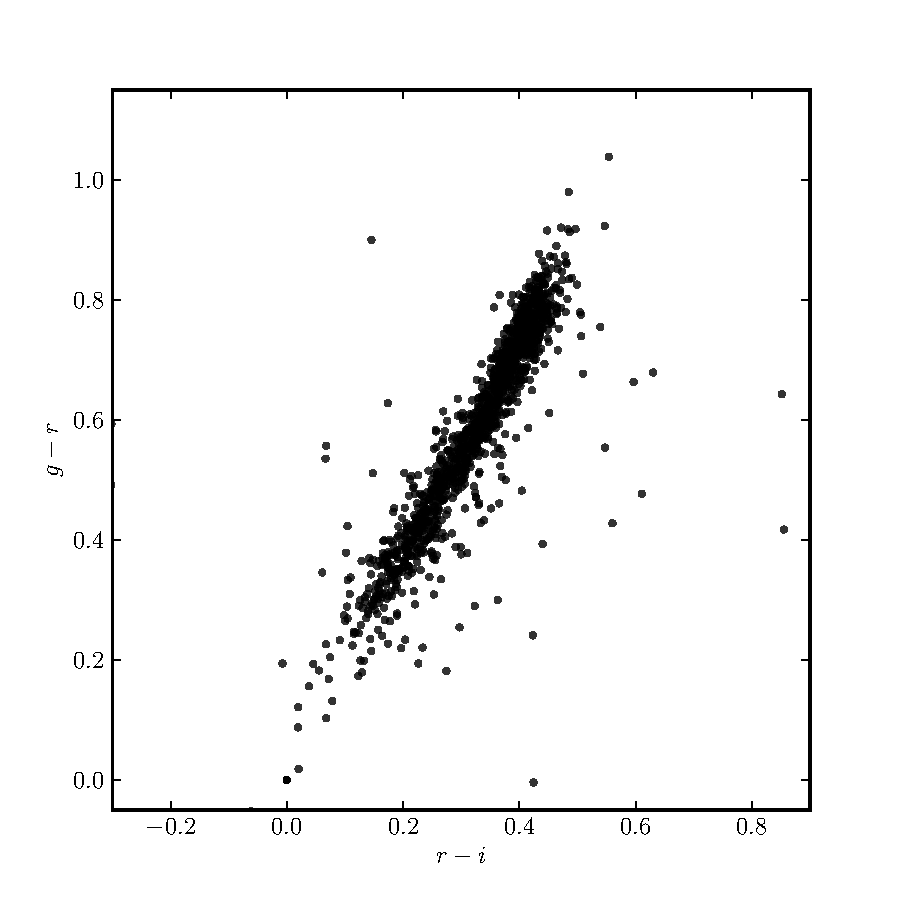
\includegraphics[trim = 15mm 0mm 0mm 0mm]{method_color_sloan.pdf}
\caption{A color-color plot of our Sloan Atlas data}
\end{figure}

\begin{figure}
\centering
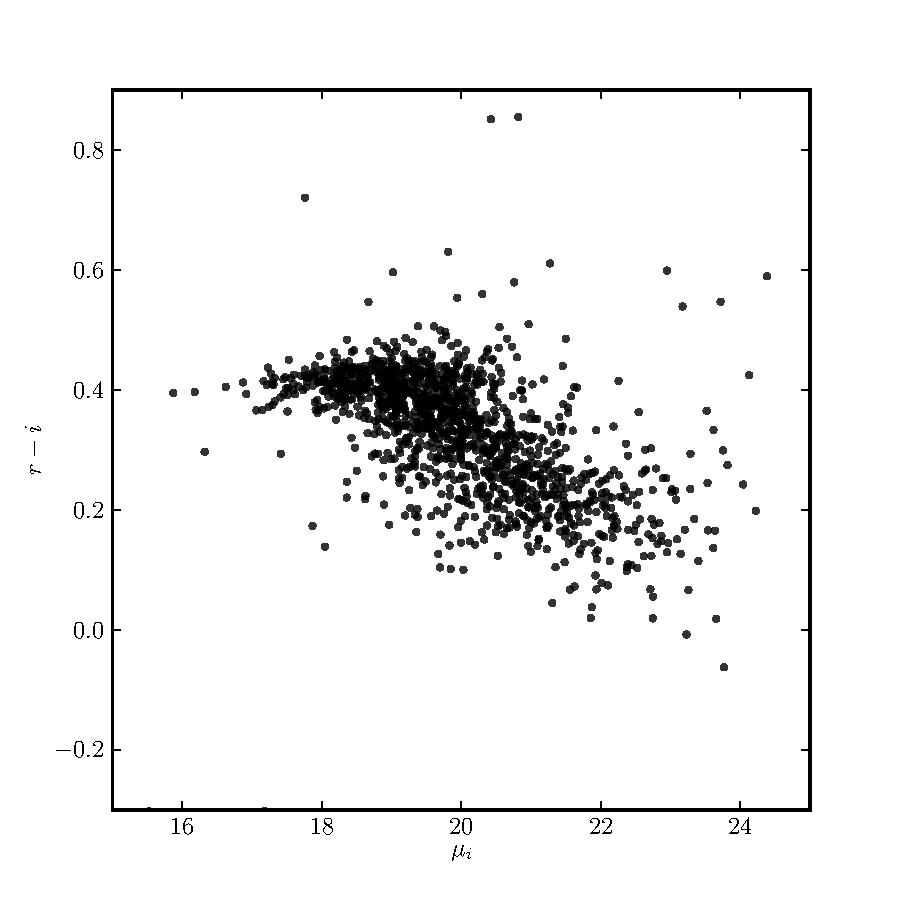
\includegraphics[trim = 15mm 0mm 0mm 0mm]{method_sb2_sloan.pdf}
\caption{Surface brightness in the i-band versus the r-i color for our Sloan Atlas data}
\end{figure}

\begin{figure}
\centering
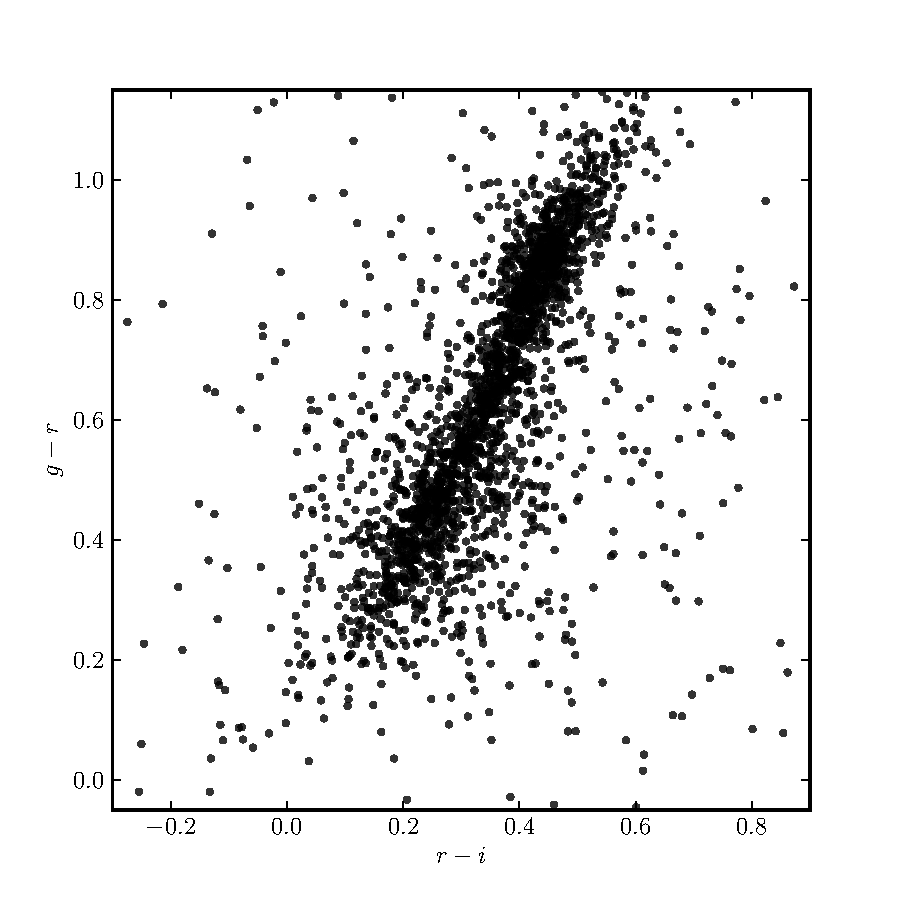
\includegraphics[trim = 15mm 0mm 0mm 0mm]{method_color_nsa.pdf}
\caption{A color-color plot of the NASA-Sloan Atlas data}
\end{figure}

\begin{figure}
\centering
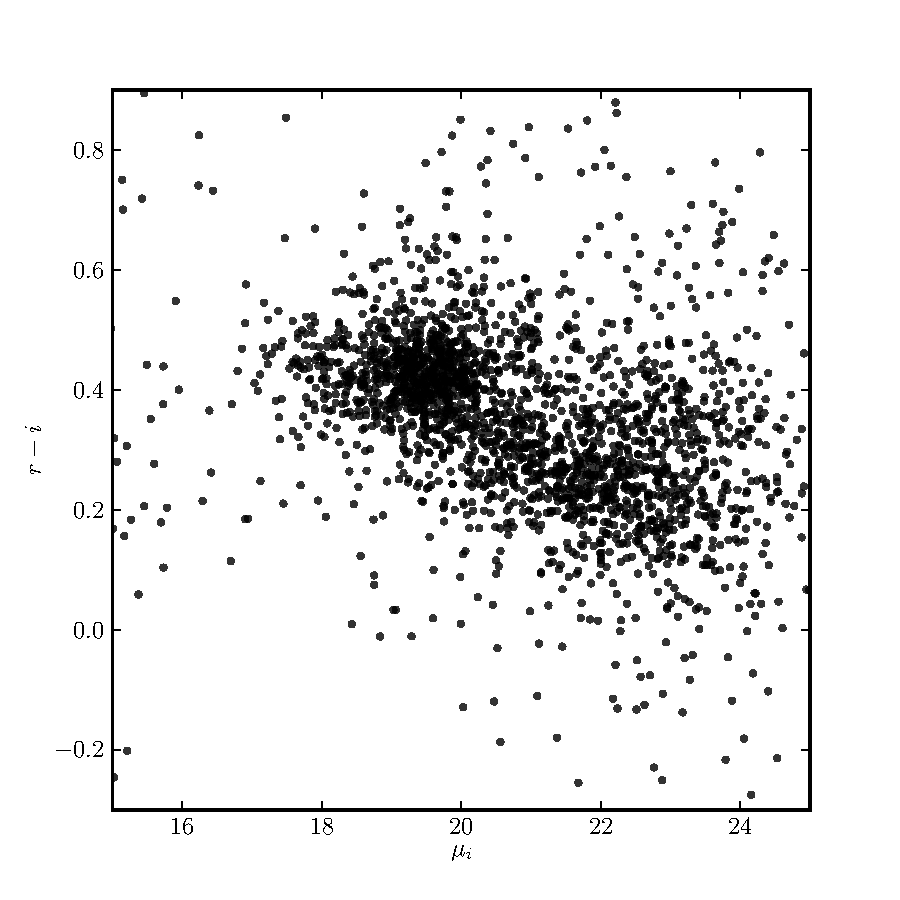
\includegraphics[trim = 15mm 0mm 0mm 0mm]{method_sb2_nsa.pdf}
\caption{Surface brightness in the i-band versus the r-i color for the NASA-Sloan Atlas data}
\end{figure}

\begin{figure}
\centering
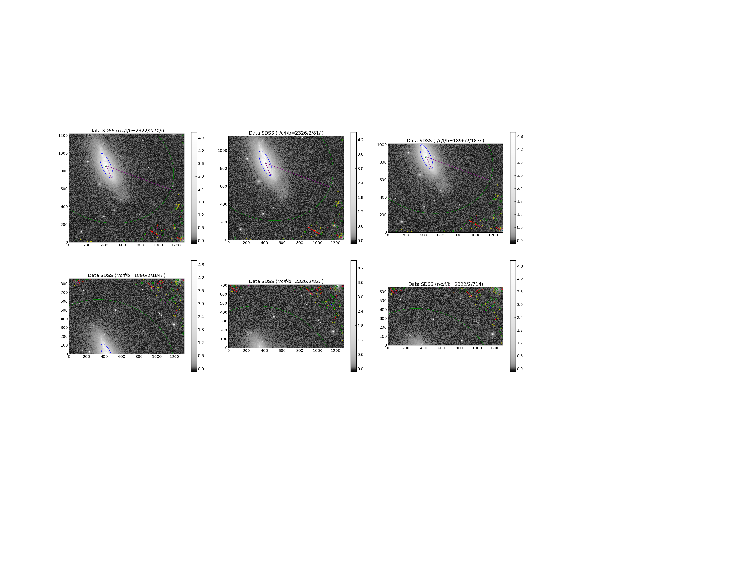
\includegraphics[trim = 1cm 3.2cm 3.8cm 2.15cm,clip=true,width=\textwidth] {data.pdf}
\caption{This shows the six different fields of data which are combined for the galaxy NGC 4605. The different fields represent different images taken by the Sloan telescope at different positions and different times.}
\label{fig:4605data}
\end{figure}
\begin{figure}
\centering
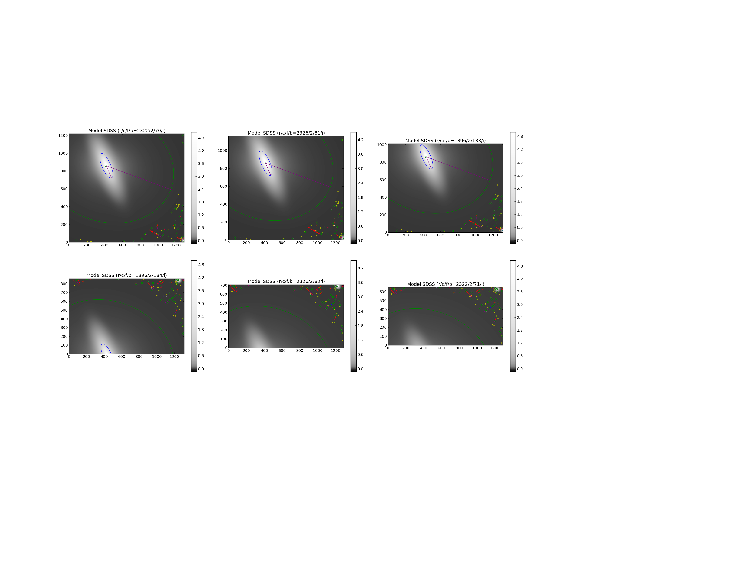
\includegraphics[trim = 1cm 3.2cm 3.8cm 2.15cm,clip=true,width=\textwidth] {model.pdf}
\caption{This is like fig \ref{fig:4605data} but shows the model we have built for the galaxy}
\label{fig:4605model}
\end{figure}
\begin{figure}
\centering
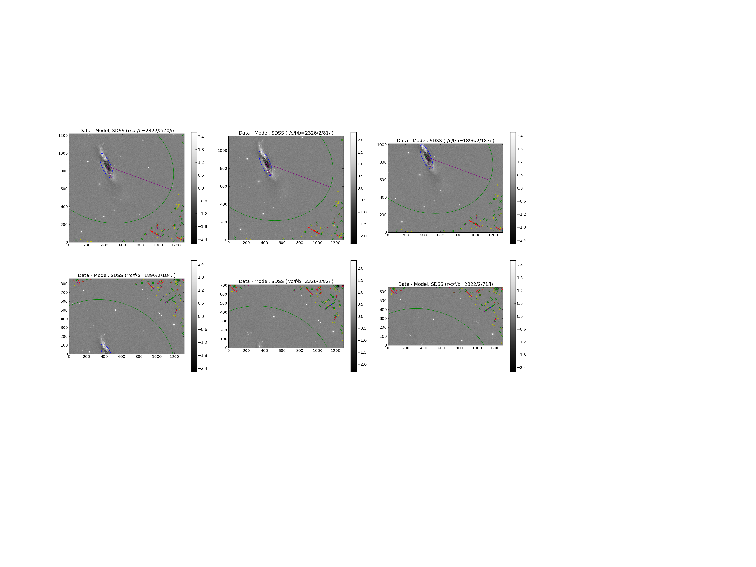
\includegraphics[trim = 1cm 3.2cm 3.8cm 2.15cm,clip=true,width=\textwidth] {diff.pdf}
\caption{This figure shows the difference between fig \ref{fig:4605data} and fig \ref{fig:4605model}}
\label{fig:4605diff}
\end{figure}
\begin{figure}
\centering
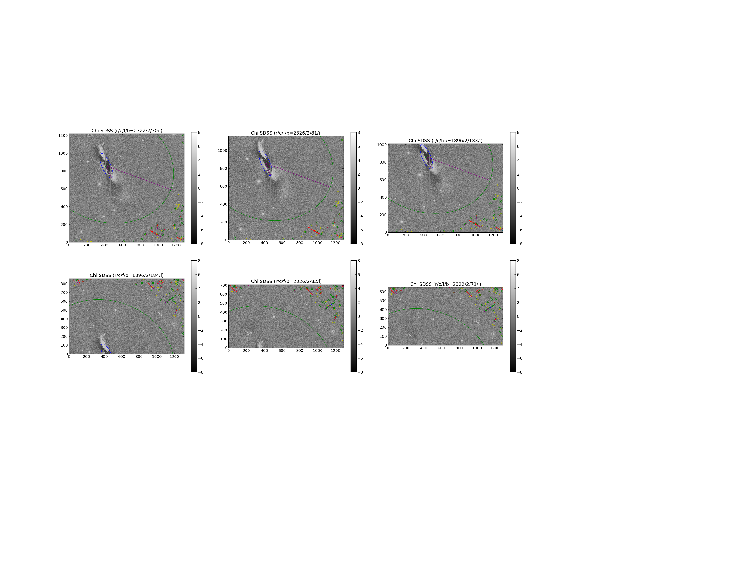
\includegraphics[trim = 1cm 3.2cm 3.8cm 2.15cm,clip=true,width=\textwidth] {chi.pdf}
\caption{This is the same as fig \ref{fig:4605diff} but shows the chi values, meaning that some pixels are masked out if they contain bad data.}
\label{fig:4605chi}
\end{figure}
\begin{figure}
\centering
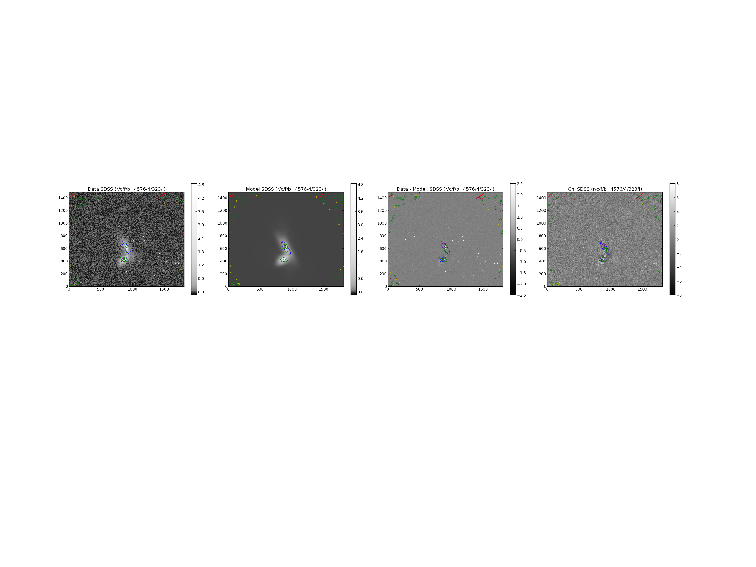
\includegraphics[trim = .9cm 4.5cm 1.15cm 2.9cm,clip=true,width=\textwidth] {gooddouble.pdf}
\caption{This figure show the fit for the galaxies NGC 3395 and NGC 3396, which are fit simultaneously. From left to right, this shows the data, the model, the residues, and the chi values in just one of the fields.}
\label{fig:gooddouble}
\end{figure}
\begin{figure}
\centering
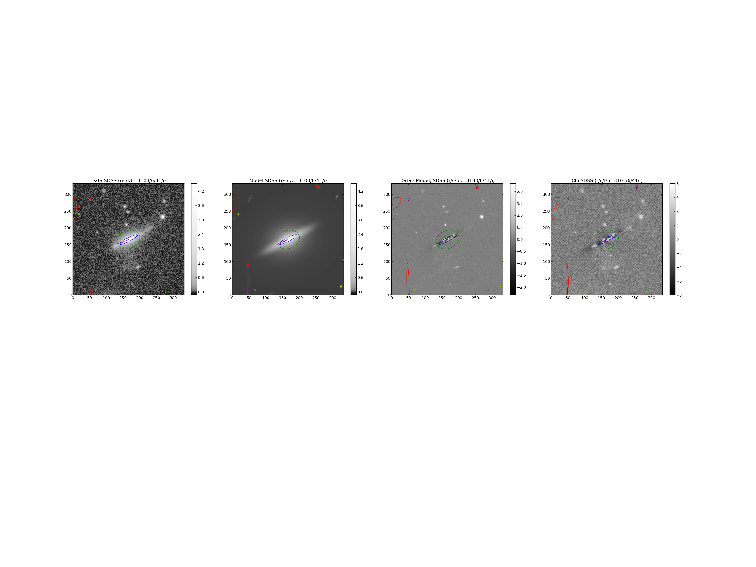
\includegraphics[trim = .9cm 4.5cm 1.15cm 2.9cm,clip=true,width=\textwidth] {badsingle.pdf}
\caption{This figure show the fit for the galaxy UGC 5613. This fit is bad because it fails to take into account that UGC 5613 is composed of a merger of two different galaxies, which causes our fit to fail. From left to right, this shows the data, the model, the residues, and the chi values in just one of the fields.}
\label{fig:badsingle}
\end{figure}
\begin{figure}
\centering
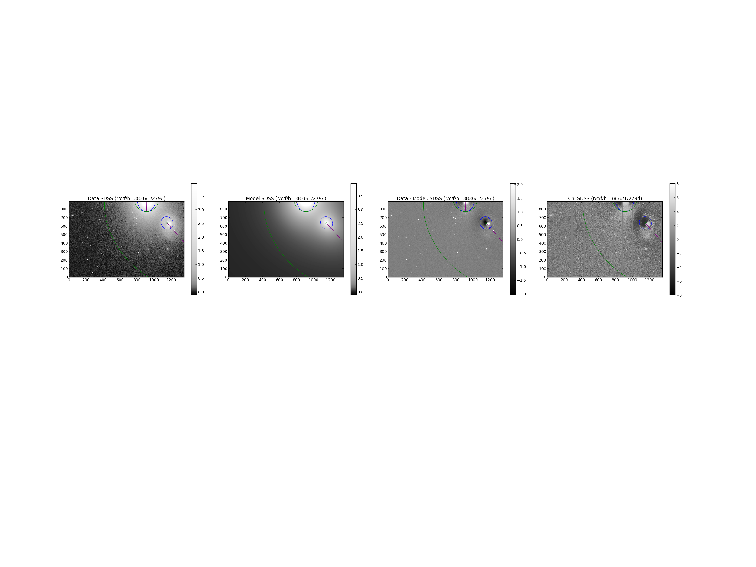
\includegraphics[trim = .9cm 4.5cm 1.15cm 2.9cm,clip=true,width=\textwidth] {baddouble.pdf}
\caption{This figure show the fit for the galaxies NGC 4647 and NGC 4649. This example shows a failure of the attempt to fit two galaxies simultaneously. From left to right, this shows the data, the model, the residues, and the chi values in just one of the fields.}
\label{fig:baddouble}
\end{figure}
\begin{figure}
\centering
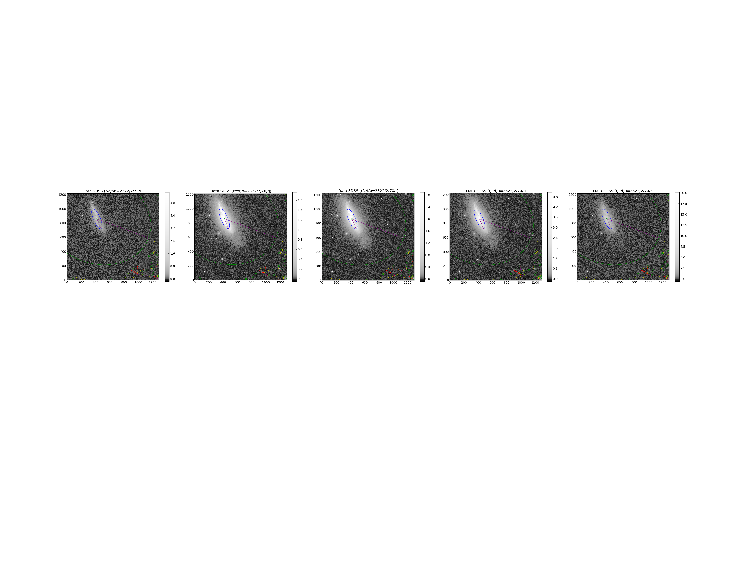
\includegraphics[trim = .9cm 4.5cm 0cm 2.9cm,clip=true,width=\textwidth] {goodsingle-colors-data.pdf}
\caption{This figure show the data for the five different bands for NGC 4605.}
\label{fig:colorsdata}
\end{figure}
\begin{figure}
\centering
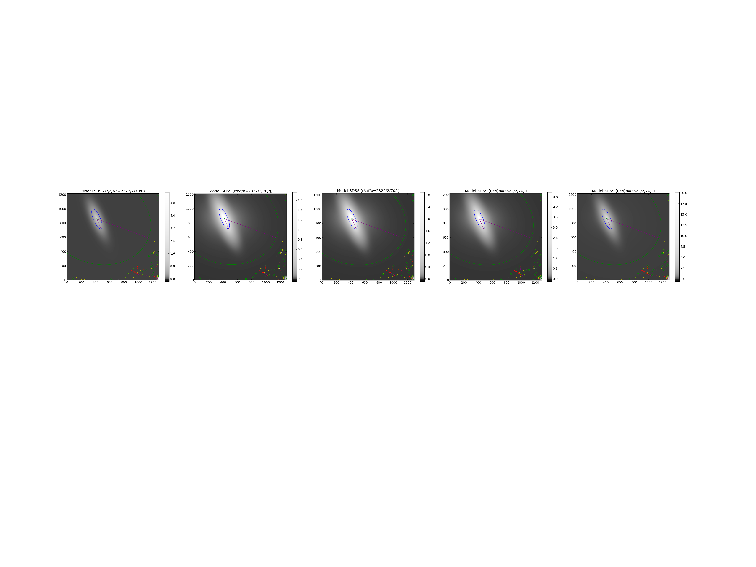
\includegraphics[trim = .9cm 4.5cm 0cm 2.9cm,clip=true,width=\textwidth] {goodsingle-colors-model.pdf}
\caption{This figure show the model for the five different bands for NGC 4605.}
\label{fig:colorsmodel}
\end{figure}
\begin{figure}
\centering
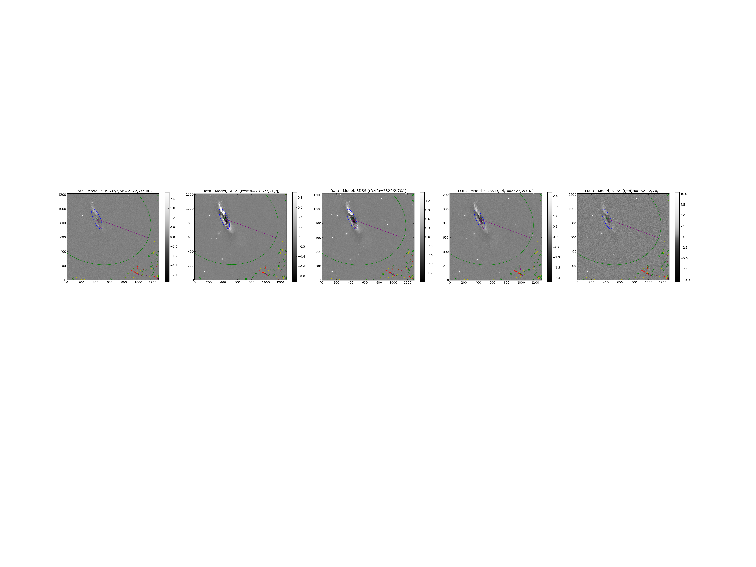
\includegraphics[trim = .9cm 4.5cm 0cm 2.9cm,clip=true,width=\textwidth] {goodsingle-colors-diff.pdf}
\caption{This figure show the diff for the five different bands for NGC 4605.}
\label{fig:colorsdiff}
\end{figure}
\begin{figure}
\centering
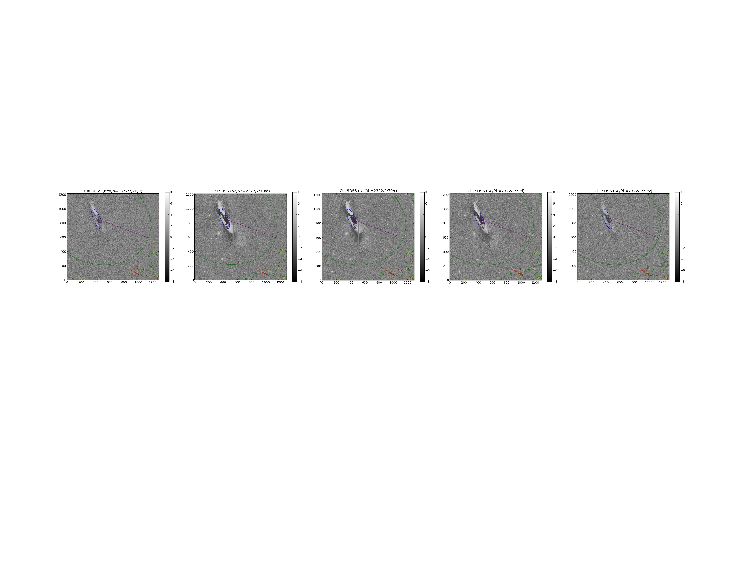
\includegraphics[trim = .9cm 4.5cm 0cm 2.9cm,clip=true,width=\textwidth] {goodsingle-colors-chi.pdf}
\caption{This figure show the chi for the five different bands for NGC 4605.}
\label{fig:colorschi}
\end{figure}
\begin{figure}
\centering
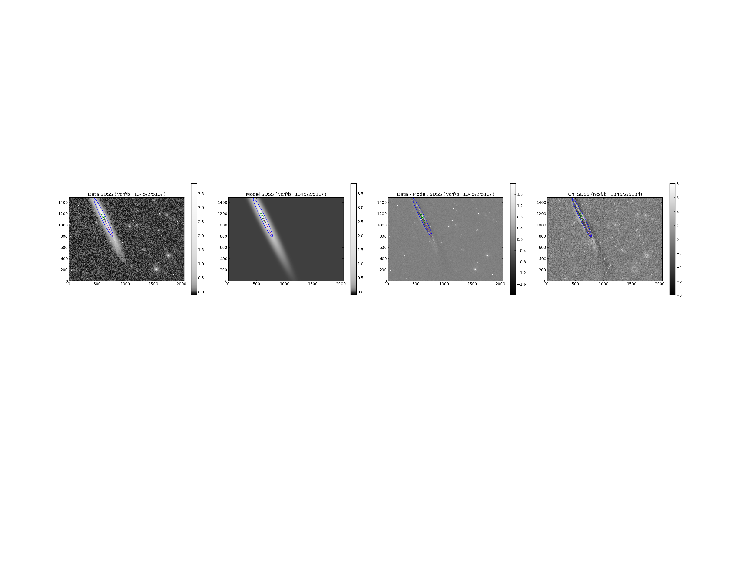
\includegraphics[trim = .9cm 4.5cm 1.15cm 2.9cm,clip=true,width=\textwidth] {edgeon.pdf}
\caption{This figure show the fit for the galaxy NGC 5907. This fit is bad because it fails on edge-on galaxies. From left to right, this shows the data, the model, the residues, and the chi values in just one of the fields.}
\label{fig:edgeon}
\end{figure}


\end{document}
